\section{Mathematisches Finanzmodell}

Wir betrachten
\begin{enumerate}[leftmargin=*]
	\item einen Wahrscheinlichkeitsraum $(\Omega, \F, \P)$, später auch weitere Maße $\Q, \dots$ auf demselben Maßraum $(\Omega, \F)$. Die $\omega \in \Omega$ werden als \begriff{Elementarereignisse} oder \begriff{''Szenarien``} bezeichnet.
	\item Zeitachse $I$ entweder $I = \menge{t_1, t_2, \dots t_N = T}$ ($N$-Perioden-Modell; diskretes Modell) oder $I = [O,T]$ (stetiges Modell)
	Dabei wird $T$ als \begriff{Zeithorizont} bezeichnet.
	\begin{definition}[stochastischer Prozess]
		Ein stochastischer Prozess $S$ ist eine messbare Abbildung 
		\begin{equation*}
		\bigabb{S}{(\Omega \times I)}{\Rd}{(\omega, t)}{S_t(\omega)}
		\end{equation*}
	\end{definition}
	Insbesondere ist 
	\begin{itemize}[nolistsep, topsep=-\parskip]
		\item $t \mapsto S_t(\omega)$ eine Funktion $I \to \Rd$ für jedes $\omega \in \Omega$ 
		\item $\omega \mapsto S_t(\omega)$ eine Zufallsvariable $\Omega \to \Rd$ für jedes $t \in I$
	\end{itemize}
	\item ~\vspace{-2em}
	 \begin{definition}[Filtration]
	 	Eine Filtration ist eine Folge von $\sigma$-Algebren $\folge{\F_t}{t \in I}$ mit der Eigenschaft
	 	\begin{equation*}
	 	\F_s \subseteq \F_t \quad \forall s,t \in I, s \le t \qquad \und \qquad \F_t \subseteq \F \quad \forall t \in I
	 	\end{equation*}
	 \end{definition}
 	\begin{*interpretation}
 		$\F_t$ beschreibt die den Marktteilnehmern zum Zeitpunkt $t$ bekannte bzw. verfügbare Information. Ein Ereignis $A \in \F_t$ gilt als \enquote{zum Zeipunkt $t$ bekannt}.
 	\end{*interpretation}
	
	\begin{*erinnerung}
		Eine $\Rd$-wertige Zufallsvariable $X$ heißt $\F_t$-messbar, wenn
		\begin{equation*}
		X^{-1}(B) \in \F_t \quad \forall \text{ Borelmengen } B \subseteq \Rd
		\end{equation*}
	\end{*erinnerung}

	\begin{beispiel}
		Sei $S$ ein stochastischer Prozess. Dann heißt
		$\F_t^S = \sigma( \menge{(S_r) : r \in I, r \le t} )$ von $S$ erzeugte Filtration.
	\end{beispiel}
	
	\begin{definition}[adaptierter Prozess]
		Ein stochastischer Prozess $\folge{S_t}{t \in I}$ auf $(\Omega, \F)$ heißt \begriff{adapiert} bezüglich einer Filtration $\folge{\F_t}{t \in I}$, wenn gilt $S_t$ ist $\F_t$-messbar für alle $t \in I$.
	\end{definition}
	
	\begin{*interpretation}
		Ist $(S_t)_{t \in I}$ ein adaptierter Prozess. Dann ist der Wert $S_t$ zum Zeitpunkt $t$ \enquote{bekannt}.
	\end{*interpretation}

	\vspace{-\parskip}
	
	Warum benötigen wir Filtrationen in der Finanzmathematik?
	\begin{itemize}[nolistsep, topsep=-\parskip]
		\item Unterscheidung zwischen Zunkunft und Vergangenheit
		\item Unterscheidung Informationen (Insider/Outsider) -- Unterscheidung Filtration $\folge{\F_t}{t \in I}$ bzw. $\folge{\G_t}{t \in I}$
	\end{itemize}
	
	\item Anlagegüter [assets]: $\R^{d+1}$-wertiger stochastischer Prozess mit Komponenten
	\begin{equation*}
		\bigabb{S^i}{(\Omega \times I)}{\R}{(\omega, t)}{S_t^i(\omega)} \quad (i \in \menge{0, 1, \dots , d})
	\end{equation*}
	$S_t^i$ beschreibt dabei den Preis des $i$-ten Anlageguts zum Zeitpunkt $t$. $S^i$ ($i \in \menge{1, \dots , d}$) ist typischerweise
	\begin{itemize}[nolistsep]
		\item Aktie [stock], Unternehmensanteil
		\item Währung [currency] bzw. Wechselkurs
		\item Rohstoff [commodity] wie z.B. Öl, Edelmetall, Elektrizität
		\item Anleihe [bond] $\dots$ Schuldverschreibung
	\end{itemize}
	
	\textbf{Hauptannahme:} $S^i$ ist liquide gehandelt (z.B. Börse), d.h. der Kauf und Verkauf zum Preis $S_t^i$ ist jederzeit möglich. 
	Der \enquote{Numeraire} $S^0$ hat eine Sonderrolle und beschreibt die Verzinsung von nicht in $(S^1, \dots , S^d)$ angelegtem Kapital. Er wird als risikolos betrachtet.
\end{enumerate}

\begin{definition}
	Ein Finanzmarktmodell (FFM) mit Zeitachse $I$ ist gegeben durch
	\begin{enumerate}[nolistsep, topsep=-\parskip]
		\item einen Wahrscheinlichkeitsraum $(\Omega, \F, \P)$ mit Filtration $\folge{\F_t}{t \in I}$
		\item einem an $\folge{\F_t}{t \in I}$ adaptierten, $\R^{d+1}$-wertigen stochastischen Prozess $S_t = (S_t^0, S_t^1 , \dots , S_t^d)$ mit $t \in I$.
	\end{enumerate}
\end{definition}
\begin{beispiel}[Cox-Ross-Rubinstein-Modell]
	Das CRR-Modell ist ein zeitdiskretes Modell beschrieben durch
	\begin{itemize}[nolistsep, topsep=-\parskip]
		\item $S_n^0 = (1+r)^n$ \dots Verzinsung mit konstanter Rate $r$
		\item $S_n^1 = S_0^1 \prod_{k=1}^n (1+R_k)$, wobei $(R_1, R_2, \dots)$ unabhängige Zufallsvariablen mit zwei möglichen Werten $a < b$ sind
	\end{itemize}

	\begin{center}
		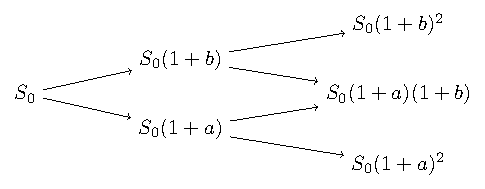
\includegraphics[width=.5\textwidth]{./img/crr-baum}
		\captionof{figure}{Cox-Ross-Rubinstein-Modell}
	\end{center}	

	Diese Darstellung nennt man einen rekombinierenden Baum; Ereignisse $\omega$ entsprechen Pfaden in diesem Baum.
\end{beispiel}

\begin{beispiel}[Black-Scholes-Modell, zeitstetig]
	Beim Black-Scholes-Modell handelt es sich um ein zeitstetiges Modell auf einem unendlichen Wahrscheinlichkeitsraum.
	\begin{equation*}
		\begin{aligned}
		S_t^0 &= e^{rt} && (\text{Verzinsung mit konstanter Rate } r) \\
		S_t^1 &= S_0^1 * \exp\brackets{(\mu-\tfrac{\sigma^2}{2}) + \sigma B_t} &&\mit \mu \in \R, \sigma > 0, S_0^1 > 0
		\end{aligned}
	\end{equation*}
	Der Term $\mu-\frac{\sigma^2}{2}$ beschreibt dabei eine Trendkomponenten, $B_t$ eine ''Brownsche Bewegung`` (zeitstetiger Prozess).
	\begin{center}
		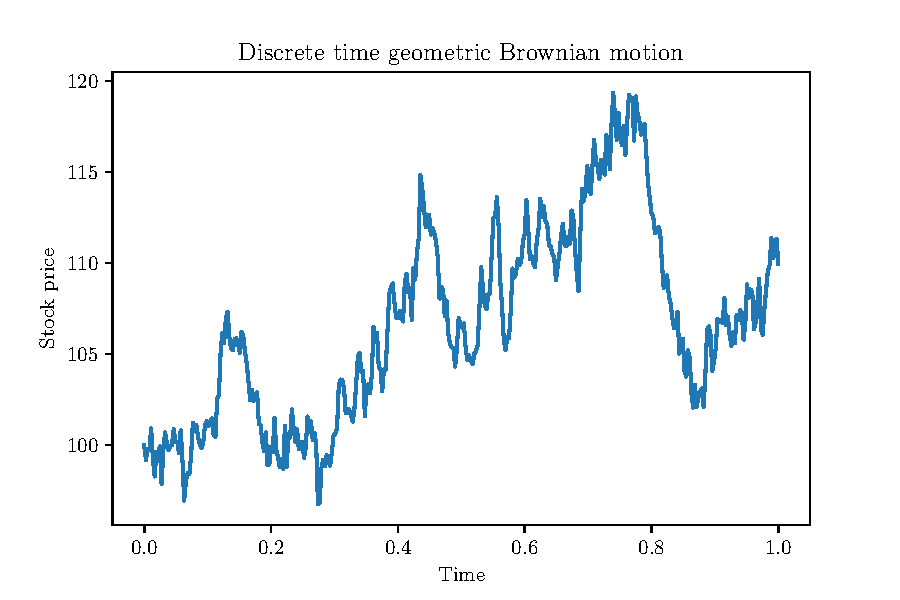
\includegraphics[width=.7\textwidth]{img/stockpricesim}
		\captionof{figure}{Black-Scholes-Modell: Simulation eines Aktienverlaufes in einem Jahr}
	\end{center}
\end{beispiel}

